\section{Export data}\label{export-data}

The data loaded in \lstinline!expVIP! can be exported to be run in
DESeq2, or any other software to do differential expression analysis.

\subsection{Wizard to export data}\label{wizard-to-export-data}

\begin{enumerate}
\def\labelenumi{\arabic{enumi}.}
\itemsep1pt\parskip0pt\parsep0pt
\item
  Double clicl on the the \lstinline!export_tables.sh! script
  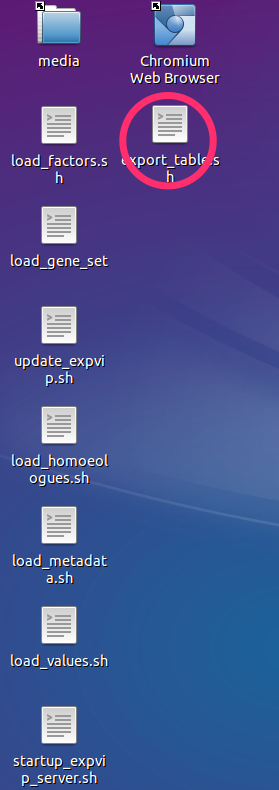
\includegraphics{images/ExportData01.png}
\item
  Execute it on the terminal 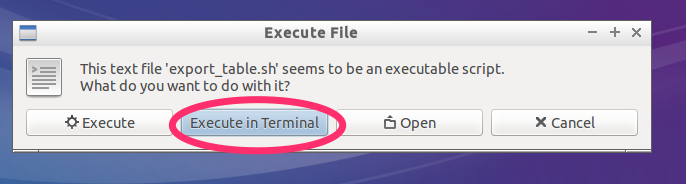
\includegraphics{images/ExportData02.png}
\item
  Select the value you want to export. If you have used
  \lstinline!Kallisto!, the available options are \lstinline!count! and
  \lstinline!tpm!. If you imported the data manually, it will be
  whatever units you inserted 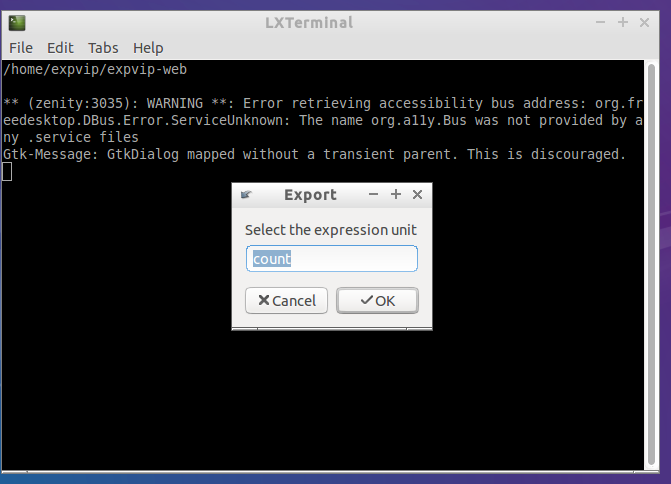
\includegraphics{images/ExportData03.png}
\item
  Select a location for the output file. It is suggested to export it in
  the shared folder with the host machine.
  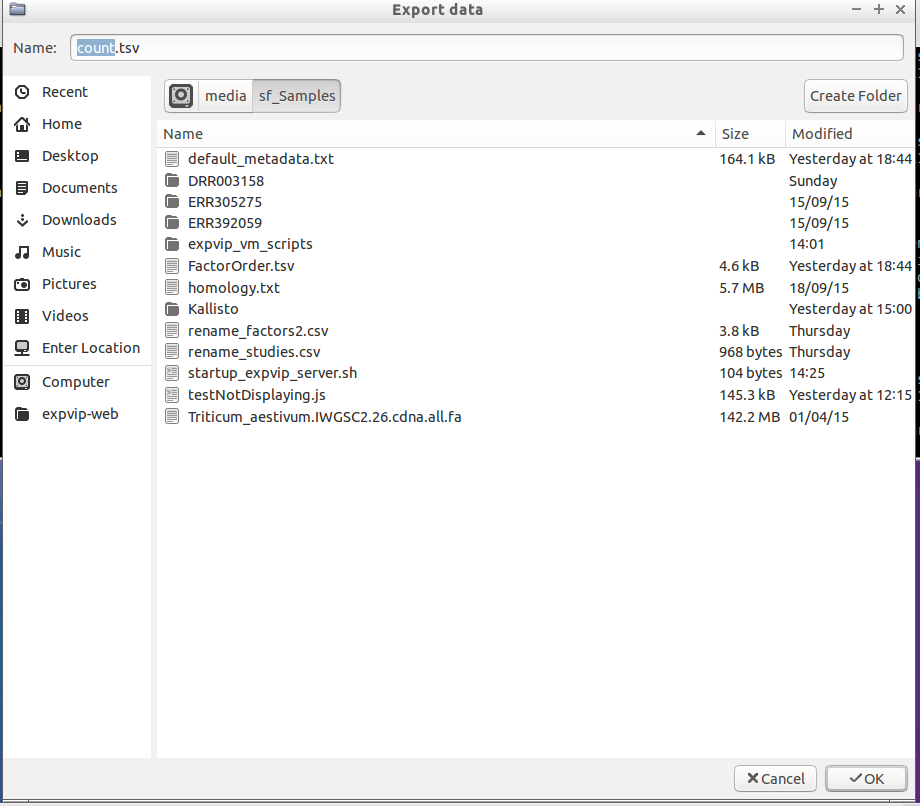
\includegraphics{images/ExportData04.png}
\end{enumerate}

\subsection{Rake tast}\label{rake-tast}

\begin{lstlisting}[language=sh]
rake "export:values[tpm,tpm.csv]"
\end{lstlisting}

\section{Abundance files}\label{abundance-files}

To use Sleuth, the abundance files from the \lstinline!Kallisto! runs
can be grabed from the folder \lstinline!kallisto! inside the folder
with reads.

The abundance files for the runs in the VM and in
\href{http://www.wheat-expression.com}{wheat-expression.com} can be
found in thie
\href{https://www.dropbox.com/sh/dap4eer67qfe9om/AADEyXZ393jY9czjAlArsemma?dl=0}{here}.

\subsection{Troublshooting}\label{troublshooting}

If you get an error like this:

\begin{lstlisting}
ActiveRecord::StatementInvalid: Mysql2::Error: Error writing file '/tmp/MYg0xdqm' (Errcode: 28 - No space left on device):
\end{lstlisting}

You can try increasing the size of the virtual machine disk or install
expVIP in a dedicated workstation. The best thing to do is to download
the precalculated tables from the expVIP website and add the columns
with your experiment at the end of the table.
